\section{Exercises}\label{4_4_exercises}
%should have predefined exercises that can be tracked in an appropriate manner
Each exercise is part of one stage. An exercise itself is divided into two body sides, which are further divided into several repetitions, see figure \ref{fig:exerciseStructure}. Each exercise is locked except the first one to provide a starting point. The next exercise can be unlocked by accomplishing both sides of the current exercise. Similarly a side is completed if all repetitions have been finished. Like for the stage, each exercise should be instructed for the user, such that she can successfully perform it. She should stand in a starting position to start the exercise. This is to ensure that no exercise is starting to track if the user would make a random gesture which could lead to confusion of the user. During the execution she should get real time feedback about her current performance, which is further discussed in \textbf{\nameref{4_6_feedbackSystem}}. After the execution a summary should show the performance of the execution with several parameters like execution time, amount of attempts needed, and the confidence regarding the given gesture.

\begin{figure}[htb]
	\centering
	\begin{minipage}[t]{1\linewidth}
		\centering
		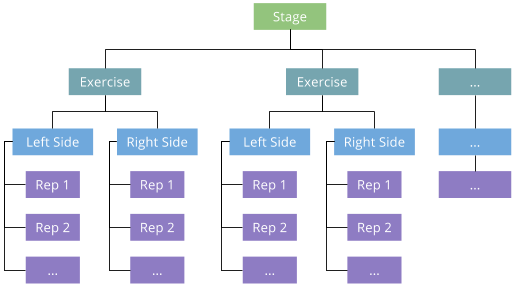
\includegraphics[width=1\linewidth]{Pictures/exerciseStructureTopDown2}
		\caption{Exercise structure}
		\label{fig:exerciseStructure}
	\end{minipage}
\end{figure}
\begin{comment}
\\\textbf{Exercises}
\\- System should provide predefined exercises that user can execute and her performance is tracked
\\- main menu / exercise selection
\\- lock / unlock 
\\- Each next exercise is unlocked if current exercise is successfully completed
\\- Each exercise counts as accomplished if both sides has been successfully trained
\\- click on exercise -> side selection - Each exercise consists of 2 sides, for train left and right side
\\- per exercise there should be an introduction on how to perform it successfully (instruction tip list, amount of repetitions, minimum time to hold a gesture, looping video)
\\- user has to stay in a starting position (both legs parallel to each other)
\\- exercise execution (user mirror)
\end{comment}
